\documentclass[fleqn]{beamer}
%\usepackage{xkeyval}
%\usepackage{todonotes}
%\presetkeys{todonotes}{inline}{}
\usepackage{xcolor}
\usepackage{tcolorbox}
%\usepackage{lipsum}
%\usepackage{xargs}
%\usepackage[pdftex,dvipsnames]{xcolor}  % Coloured text etc.

\usepackage{tabularx}
\usepackage{booktabs}
\usepackage{colortbl}
\usepackage{tikz}
\usetikzlibrary{calc}
\pgfdeclarelayer{background}
\pgfdeclarelayer{foreground}
\pgfsetlayers{background,main,foreground}
%\setbeamertemplate{background canvas}[vertical shading]%
%  [top=blue!1,bottom=blue!30]
\setbeamertemplate{navigation symbols}{}
\newcommand*\up{\textcolor{green}{%
  \ensuremath{\blacktriangle}}}
\newcommand*\down{\textcolor{red}{%
  \ensuremath{\blacktriangledown}}}
\newcommand*\const{\textcolor{darkgray}%
  {\textbf{--}}}

\newcounter{todo}
\newtcbox{\mytodobox}{colback=orange,colframe=orange!75!black}

 \newcommand\todo[1]{%
     \refstepcounter{todo} 
    \mytodobox{\hypertarget{todo\thetodo}{#1}}
     \addcontentsline{tod}{subsection}{\protect\hyperlink{todo\thetodo}{\thetodo~#1}\par} 
 }%

\makeatletter
\newcommand\listoftodos{%
    \@starttoc{tod}}
\makeatother

\usepackage{graphicx,ksu,url}
\usepackage{amsmath}
% Use Times for math font and text font.
\RequirePackage[T1]{fontenc}
%\RequirePackage{txfonts}
% bold math must be loaded after Times font
\usepackage{bm}
\usepackage{booktabs} % nice rules (thick lines) for tables
\usepackage{microtype} % improves typography for PDF
\usepackage{xcolor} % Allows colors in fonts
\usepackage{tikz} % Allows creation of tikz pictures
\usepackage{verbatim}
\usepackage{fancyvrb}
\usepackage{mathalfa}
\usepackage{mathrsfs}
\DeclareMathOperator*{\argmin}{argmin}
\DeclareMathAlphabet{\mathpzc}{OT1}{pzc}{m}{bf}
\renewcommand{\vec}[1]{\bm{#1}} %vector is bold italic
\newcommand{\vd}{\bm{\cdot}} % slightly bold vector dot
\newcommand{\grad}{\vec{\nabla}} % gradient
\newcommand{\ud}{\mathop{}\!\mathrm{d}} % upright derivative symbol
\graphicspath{{../../data/images/}}

\usepackage{etoolbox}
\AtBeginEnvironment{quote}{\singlespacing\small}

\usetikzlibrary{arrows,shapes}
\usetikzlibrary{decorations.pathreplacing,matrix, positioning}
\setlength\intextsep{1\baselineskip plus 3pt minus 2 pt}
%\usepackage{minted} % Allows printing of python (or other) code
%\newminted{python}{fontsize=\scriptsize, 
%    linenos,
%    numbersep=8pt,
%    gobble=4,
%    frame=lines,
%    bgcolor=bg,
%    framesep=3mm}

% The title of the presentation:
%  - first a short version which is visible at the bottom of each slide;
%  - second the full title shown on the title slide;
\title[]{
    Analysis of the LRA Reactor Benchmark Using Dynamic Mode Decomposition}

% Optional: a subtitle to be displayed on the title slide
%\subtitle{Show where you're from}

% The author(s) of the presentation:
%  - again first a short version to be displayed at the bottom;
%  - next the full list of authors, which may include contact information;
\author[]{
Dr. Mohammad Abdo \\
	       Rabab Elzohery \\
               Prof. Jeremy Roberts}

% The institute:
%  - to start the name of the university as displayed on the top of each slide
%    this can be adjusted such that you can also create a Dutch version
%  - next the institute information as displayed on the title slide
\institute[Kansas State University]{
    Mechanical and Nuclear Engineering \\
    Kansas State University}

% Add a date and possibly the name of the event to the slides
%  - again first a short version to be shown at the bottom of each slide
%  - second the full date and event name for the title slide

\date[]{\emph{{\textbf{2018 ANS Winter Meeting and Nuclear Technology Expo, "Joining Forces to Advance Nuclear"}}
    November 11-15- 2018}}

\begin{document}
    % These two commands allow bonus slides at the end
    % The bonus slides will not be numbered
    \newcommand{\beginbackup}{
        \newcounter{framenumbervorappendix}
        \setcounter{framenumbervorappendix}{\value{framenumber}}
    }
    \newcommand{\backupend}{
        \addtocounter{framenumbervorappendix}{-\value{framenumber}}
        \addtocounter{framenumber}{\value{framenumbervorappendix}} 
    }
    
    \begin{frame}
        \titlepage
    \end{frame}
    

\section{Background and Motivation}
    
    
%%%%%%%%%%%%%%%%%%%%%%%%%%%%%%%%%%%%%%%%%%%%%%%%%%%%%%%%%%%%%%%%%%%%%%%%%%%%%%%
\begin{frame}
\frametitle{A Need for Uncertainty Quantification of Transients}       

\vfill

Growing interest in transient phenomena have led to new experiments and renewed capabilities:
\pause
\begin{itemize}
 \item multiple fission chambers deployed in UWNR for a variety of  steady-state and transient reaction-rate measurements
 \pause 
 \item recent restart of TREAT is already generating new core data, with much more to follow.
\end{itemize}

\vfill 
\pause 

Analysis of experiments may required the use of advanced tools (e.g., MAMMOTH/Rattlesnake + other creatures)

\pause 
\vfill

{\bf ...but what's the uncertainty in computed results?}
 
\pause 
\vfill

Possible options:
\begin{itemize}
 \item brute-force sampling (expensive)
 \item {\bf reduced order modeling (cheap)}
\end{itemize}
 
\vfill
 
\end{frame}


%%%%%%%%%%%%%%%%%%%%%%%%%%%%%%%%%%%%%%%%%%%%%%%%%%%%%%%%%%%%%%%%%%%%%%%%%%%%%%%
\begin{frame}
    
\frametitle{Reduced Order Modeling}

Main idea: Let
\begin{equation*}
 \vec{f}(\vec{x})\approx \vec{g}(\mathcal{M}(\vec{x}))
\end{equation*}
where $\vec{x} \subseteq \mathbb{R}^n$, $\mathcal{M}(\vec{x}) \in \mathbb{R}^{r_x}$ and $r_x \ll n$.

\pause
\vfill

A large class of approximations projects underlying model onto basis (think proper-orthogonal decomposition or POD).

\pause
\vfill 

Present goal is a completely data-driven surrogate based on Dynamic Mode Decomposition (DMD).

\end{frame}


\section{Dynamic Mode Decomposition}

%%%%%%%%%%%%%%%%%%%%%%%%%%%%%%%%%%%%%%%%%%%%%%%%%%%%%%%%%%%%%%%%%%%%%%%%%%%%%%%
\begin{frame}
\frametitle{DMD Overview}


DMD was first used to analyze fluid dynamics experiments (P.J. Schmid, J. Fluid Mech. {\bf 656}), and most recent advanced summarized in a recent monograph (N. Kutz {\it et al.}, SIAM).

\pause
\vfill

Some scoping work in nuclear with applications of DMD to:
\begin{itemize}
 \item modeling nuclide evolution (Abdo {\it et al.})
 \item decay heat generation (Alfonsi, {\it et al.})
\end{itemize}
Maybe others?

% \begin {itemize}
% \item DMD first used by Schmid in 2008, in fluid dynamics \cite{schmid08}.
% \item It is used to explore the behavior of dynamical systems.\footnote{lalal}
% \item  It can be viewed as a PCA (spatial domain) + DFT (frequency domain).
% % \item  It can be viewed as a combination of a PCA in the spatial domain and Discrete Fourier Transform (DFT) in the frequency domain.
% 
% \end{itemize}

\end{frame}


%%%%%%%%%%%%%%%%%%%%%%%%%%%%%%%%%%%%%%%%%%%%%%%%%%%%%%%%%%%%%%%%%%%%%%%%%%%%%%%
\begin{frame}
\frametitle {DMD Methodology}

Consider a dynamical system described by $\frac{d\mathbf{y}}{dt} = \mathbf{f}(\mathbf{y}, t)$. 

\vfill 
\pause

Suppose one makes successive measurements spaced by $\Delta t$ that lead to the $m\times n$ matrices

\begin{equation*}
\mathbf{Y_0}=\left[\begin{array}{ccc}
| & |   & | \\
{\vec{y_0}} &   ... & {\vec{y_{n-1}}} \\ 
| & | &  | 
\end{array} \right] 
 \,\, \text{and} \quad
{\mathbf{Y_1}}=
\left[\begin{array}{ccc}
| & |  & | \\ 
{\vec{y_1}} & ... & {\vec{y_{n}}} \\ 
| & |  & |
\end{array} \right]\, .
\end{equation*}

\vfill 
\pause

Koopman once showed there is an infinite-dimensional $\mathcal{A}$ that maps $\mathbf{y}_{i}$ to $\mathbf{y}_{i+1}$.  
Here, we seek the {\it finite} operator $\mathbf{A}$ that best satisfies
\begin{equation*}
   \mathbf{Y_1} \approx \mathbf{A} \mathbf{Y_0} \, .
\end{equation*}

\end{frame}

%%%%%%%%%%%%%%%%%%%%%%%%%%%%%%%%%%%%%%%%%%%%%%%%%%%%%%%%%%%%%%%%%%%%%%%%%%%%%%%
\begin{frame}
\frametitle{DMD Methodology}

Specifically, seek $\mathbf{A}$ that fits the data in a least-squares sense, or 

\begin{equation*}
\mathbf{A}=\argmin\limits_{\mathbf{A}}\|\mathbf{Y_{1}} -\mathbf{AY_{0}}\|_F = \mathbf{Y_1}\mathbf{Y_0^{+}} \, .
\end{equation*}

\vfill 
\pause
 
In practice, $\mathbf{A}$  is very large, so DMD uses a low-rank approximation based on the singular value decomposition (SVD).
\vfill
\end{frame}


%%%%%%%%%%%%%%%%%%%%%%%%%%%%%%%%%%%%%%%%%%%%%%%%%%%%%%%%%%%%%%%%%%%%%%%%%%%%%%%
\begin{frame}
\frametitle{Singular Value Decomposition}

 
The SVD is exploited to reveal the low dimensional structure in the data by keeping the first $r$ singular values that recovers most of the data variance, i.e.,
\begin{equation*}
 \mathbf{Y_0} \approx \mathbf{U_r}\boldsymbol{\Sigma}_{\mathbf{r}}\mathbf{V_r^{H}} \, .
\end{equation*}


The columns of {$\mathbf{U_r}$} are the {\bf POD} modes onto which the data will be projected.  


\end{frame}

%%%%%%%%%%%%%%%%%%%%%%%%%%%%%%%%%%%%%%%%%%%%%%%%%%%%%%%%%%%%%%%%%%%%%%%%%%%%%%%
\begin{frame}
\frametitle{Basic DMD Algorithm}

Starting with SVD of $\mathbf{Y}_0$, do
\begin{enumerate}
 \pause
 \item 
 \begin{tabular}{p{6cm}r}
  $\mathbf{U_r^{H}Y_1} = \mathbf{U_r^H}\mathbf{A}\mathbf{Y_0} =  \underbrace{\mathbf{U_r^{H} A U_r}}_{\tilde{\mathbf{A}}}\boldsymbol{\Sigma}\mathbf{_r}\mathbf{V_r^{H}}.$
    &  \pause $\mathbf{A}$ and $\mathbf{\tilde{A}}$ are similar. \\
 \end{tabular}
 \pause
 \item 
 \begin{tabular}{p{5cm}r}
  $\mathbf{\tilde{A}}=\mathbf{U_r^{H}Y_1}\mathbf{V_r}\boldsymbol{\Sigma}_{\mathbf{r}}^{-1}.$
    &   \\
 \end{tabular}
 \pause
 \item 
 \begin{tabular}{p{5cm}r}
   $\mathbf{\tilde{A} \tilde{W}}=\mathbf{\tilde{W}}\boldsymbol{\Lambda}$ 
    &    \\
 \end{tabular}
 \pause
 \item 
 \begin{tabular}{p{5cm}r}
    $\omega_i= \text{log}(\lambda_i)/\Delta t.$
    &  \pause discrete to continuous \\
 \end{tabular}
 \pause
 \item 
 \begin{tabular}{p{5cm}r}
   ${\boldsymbol{\Phi}}={\mathbf{Y_1 V_r}}\boldsymbol{\Sigma}_\mathbf{r}^{-1}{\mathbf{\tilde{W}}}.$
    &  \pause the ``DMD modes'' \\
 \end{tabular}
%  \item 
%  \begin{tabular}{lr}
%   $\vec{x}^{DMD}(t)\approx \sum_{i=1}^{r} b_i \boldsymbol{\phi}_i^{DMD} e^{\omega_it}={{\boldsymbol{\Phi}}}^{DMD}{\mathbf{diag}}(e^{\vec{\omega}t})\vec{b}$
%     &  \pause The surrogate \\
%  \end{tabular}
\end{enumerate}

% \pause
% \begin{block}{The surrogate}
% $\vec{y}^{DMD}(t)\approx \sum_{i=1}^{r} b_i \boldsymbol{\phi}_i e^{\omega_it}={{\boldsymbol{\Phi}}} \, {\textrm{diag}}(e^{\vec{\omega}t})\vec{b}$
% \end{block}

\end{frame}

\begin{frame}
\frametitle{Reconstruction and the Surrogate}

Given $\mathbf{\phi}$ and $w_i$, define the DMD surrogate
\begin{equation*}
 \vec{y}^{DMD}(t)\approx \sum_{i=1}^{r} \textcolor{blue}{b}_i \boldsymbol{\phi}_i e^{\omega_it}={{\boldsymbol{\Phi}}} \, {\textrm{diag}}(e^{\vec{\omega}t})\vec{\textcolor{blue}{b}} \, ,
\end{equation*}
but what about $\mathbf{b}$?


\vfill 
\pause

The (maybe) obvious definition: $\mathbf{b} = \boldsymbol{\Phi}^+ \mathbf{y}_0$.

\vfill 
\pause 

Other options: set $\mathbf{b}$ to minimize $||\mathbf{Y}^{DMD} - \mathbf{Y}||_F$ or the method by Jovanovic {\it et al}.


\vfill

\end{frame}

\begin{frame}
\frametitle{Partitioned DMD}


Basic DMD does poorly for large transients, and adding modes (non-orthogonal) not guaranteed to increase accuracy.

\vfill 
\pause

A potential solution: {\bf define time partitions each with its own surrogate and feed output of one to the next}.

\vfill 
\pause

Here, all partitioning is {\it ad hoc}, but variable that could be formally optimized include
\begin{enumerate}
 \item number of partitions
 \item partition boundaries
 \item partition rank (i.e., how many modes in each)
 \item mode amplitudes
\end{enumerate}

\end{frame}


%%%%%%%%%%%%%%%%%%%%%%%%%%%%%%%%%%%%%%%%%%%%%%%%%%%%%%%%%%%%%%%%%%%%%%%%%%%%%%%

\begin{frame}

\frametitle{LRA Benchmark: Laboratorium f{\"u}r Reaktorregelung und Anlagensicherung}       

\begin{itemize}
  \item 2D LRA benchmark is a 2-group, quarter-core BWR.
  \item Simplicity of the geometry renders the problem tractable personal computers
  \item  It was used to test modern neutronics codes.        
    \item assemply homogenized cross section data
    \item ramp absorption cross section is simulation control rod ejection
    \item Originally posed as a diffusion problem, solved with coarse mesh and nodel diffusion methods.
    \item Scruntinizes the reactivity insertion accedent. 
       
\end{itemize}

\end{frame}

    
\begin{frame}

\frametitle{DETRAN:}       
\begin{itemize}
       \item A DEterministic TRANsport code originally developed by Jermey Roberts.
       \item It utilizes methods such as Multigroup diffusion, discrete ordinates, MOC.
       \item features solvers for fixed source and eigenvalue problems including preconditioned-Krylov linear solvers. 
%         
    \item For this work, 2-group diffusion was employed to provide the data, hereinafter refered to as the high fidelity data.
       
  
       \end{itemize}
    \end{frame}


    \section{Actual Model Description}

    \begin{frame}
        \frametitle{Physical Model}
        \begin{columns}[c]
            \begin{column}{0.7\textwidth} 
\begin{figure}
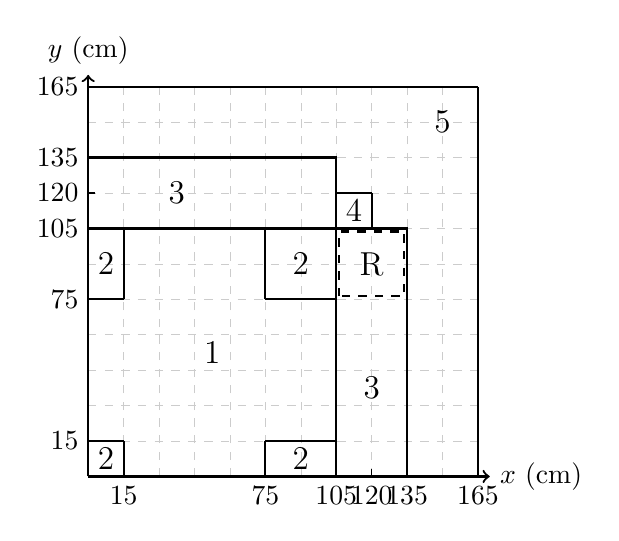
\begin{tikzpicture}[scale=.3]

\begin{scope}<->;

% GRID
  \draw[step=1.5cm,gray,very thin, dashed,opacity=0.4] (0, 0) grid (16.5,16.5);

% AXES
  \draw[black, thick, ->] (0, 0) -- (17,  0) node[right] {$x$ (cm)};
  \draw[black, thick, ->] (0, 0) -- ( 0, 17) node[above] {$y$ (cm)};

% Material 1 regions 

  \node[font=\large] at (5.25, 5.25) {1};
  
% Material 2 regions
  \draw[black, thick] (0, 1.5) -- (1.5, 1.5);
  \draw[black, thick] (1.5, 0) -- (1.5, 1.5);
  \node[font=\large] at (0.75, 0.75) {2};
  
  \draw[black, thick] ( 7.5, 0.0) -- ( 7.5, 1.5);
  \draw[black, thick] (10.5, 0.0) -- (10.5, 1.5);
  \draw[black, thick] ( 7.5, 1.5) -- (10.5, 1.5);
  \node[font=\large] at (9.0, 0.75) {2};

  \draw[black, thick] ( 0.0,  7.5) -- ( 1.5,  7.5);
  \draw[black, thick] ( 0.0, 10.5) -- ( 1.5, 10.5);
  \draw[black, thick] ( 1.5,  7.5) -- ( 1.5, 10.5);
  \node[font=\large] at ( 0.75, 9.0) {2};
  
  \draw[black, thick] ( 7.5,  7.5) -- ( 7.5, 10.5);
  \draw[black, thick] ( 7.5,  7.5) -- (10.5,  7.5);
  \draw[black, thick] (10.5, 10.5) -- ( 7.5, 10.5);
  \draw[black, thick] (10.5, 10.5) -- (10.5,  7.5);
  \node[font=\large] at ( 9.0, 9.0) {2};

% Material 3 regions
  \draw[black, thick] (10.5,  0.0) -- (10.5, 10.5) -- (13.5, 10.5) --  (13.5,  0.0) -- (10.5,  0.0);
  \node[font=\large] at ( 12.0, 3.75) {3}; 
  \draw[black, thick] (0.0, 10.5) -- (10.5, 10.5) -- (10.5, 13.5) -- (0.0, 13.5) --  (0.0, 10.5);
  \node[font=\large] at ( 3.75, 12.0) {3}; 
  
% Material 4 regions  
  \draw[black, thick] ( 12,  12) -- ( 12, 10.5) -- (10.5, 10.5) -- (10.5,  12) -- ( 12,  12);
  \node[font=\large] at ( 11.25,11.25) {4};

   
% Material 5 regions
  \draw[black, thick] ( 16.5,  0.0) -- (16.5, 16.5);
  \draw[black, thick] (  0.0, 16.5) -- (16.5, 16.5);
  \node[font=\large] at (15.0, 15.0) {5};
 
% Perturbed regions
  \def\eps{0.125}
  \draw[black, thick, dashed] (10.5+\eps, 7.5+\eps) -- (10.5+\eps, 10.5-\eps) -- (13.5-\eps, 10.5-\eps) -- (13.5-\eps, 7.5+\eps) --  (10.5+\eps, 7.5+\eps);

  %\draw[black, thick] ( 12,  12) -- (10.5,  12);
  %\draw[black, thick] (10.5, 10.5) -- ( 12, 10.5);
  %\draw[black, thick] (10.5, 10.5) -- (10.5,  12);
  \node[font=\large] at (12,9) {R};
 
% ticks
  \foreach \x/\xtext in {15, 75, 105, 120, 135, 165}
      \draw[black,xshift=0.1*\x cm] (0,.3) -- (0,0) node[below] {$\xtext$};
  \foreach \y/\ytext in {15, 75, 105, 120, 135, 165}
      \draw[black,yshift=0.1*\y cm] (.3,0) -- (0,0) node[left] {$\ytext$};
\end{scope}
\end{tikzpicture}
\end{figure}
            \end{column}            
            \begin{column}{0.4\textwidth} 
                             \begin{block}{Model Description}              
 \begin{itemize}     
                    \item Super Prompt-critical Transient. 
                    \item 2D Diffusion.
                    \item Adiabatic Heatup and Doppler Feedback in thermal reactor.
                    
                    \end{itemize}
                \end{block}
            \end{column}
        \end{columns}
    \end{frame}
    \begin{frame}
    \frametitle{Governing Equations}
\begin{block}{2D Diffusion with two Delayed Neutron Precursor groups.}

	\begin{align*}
	\label{eq:Diffusion}
	& \nabla D_1(\vec{x},t)\nabla \phi_1(\vec{x},t)-[\Sigma_{a1}(\vec{x},t)+\Sigma_{1\rightarrow2}(\vec{x},t)]\phi_1(\vec{x},t)\\
	& +\nu( 1- \beta )[\Sigma_{f1}(\vec{x},t)\phi_1(\vec{x},t)+\Sigma_{f2}(\vec{x},t)\phi_2(\vec{x},t)]\\
	& +\Sigma_{i=1}^{2}\lambda_i c_i (\vec{x},t)=\frac{1}{v_1}\frac{\partial}{\partial t}\phi_1(\vec{x},t).\\
	& \nabla D_2(\vec{x},t)\nabla \phi_2(\vec{x},t)-\Sigma_{a2}(\vec{x},t)\phi_2(\vec{x},t)+\Sigma_{1\rightarrow2}(\vec{x},t)\phi_1(\vec{x},t)\\
	& =\frac{1}{v_2}\frac{\partial}{\partial t}\phi_2(\vec{x},t).\\
	& \nu\beta_i[\Sigma_{f1}(\vec{x},t)\phi_1(\vec{x},t)+\Sigma_{f2}(\vec{x},t)\phi_2(\vec{x},t)]-\lambda_ic_i(\vec{x},t)\\
	&=\frac{\partial}{\partial t}c_i(\vec{x},t), \ i=1,2.
	\end{align*}
\end{block}
\end{frame}
\begin{frame}
\begin{block}{Adiabatic Heatup}
\begin{equation*}
\alpha[\Sigma_{f1}(\vec{x},t)\phi_1(\vec{x},t)+\Sigma_{f2}(\vec{x},t)\phi_2(\vec{x},t)]=\frac{\partial}{\partial t}T(\vec{x},t).
\end{equation*}
\end{block}

\begin{block}{Doppler Feedback}
\begin{equation*}
\Sigma_{a1}(\vec{x},t) = \Sigma_{a2}(\vec{x},t=0)[1+\gamma(\sqrt(T(\vec{x},t))-\sqrt(T_0))].
\end{equation*}
\end{block}

\begin{block}{Power}
\begin{equation*}
P(\vec{x},t)=\varepsilon [\Sigma_{f1}(\vec{x},t)\phi_1(\vec{x},t)+\Sigma_{f2}(\vec{x},t)\phi_2(\vec{x},t)].
\end{equation*}
\end{block}
\end{frame}
% * <mgabdo@ksu.edu> 2018-03-28T13:53:50.537Z:
%
% ^.



\section{Numerical Experiments and Results}
\begin{frame}
\frametitle{Case Study}
\begin{itemize}
\item Building a surrogate for the responses of interest: i.e., Power, flux, and/or temperature.

\item 300 snapshots.
\item $22 \times 22$ spatial cells.
\item 3 seconds simulation time.
\item control rod:
\begin{equation*}
    \frac{\Sigma_{a2}(t)}{\Sigma_{a2}(0)}=\left\{
\begin{array}{ll}
1-0.0606184 \ t & t\le 0.2 \ \ sec\\
0.878763 & t>0.2 \ \ sec\\
\end{array} \right. 
\end{equation*}

\end{itemize}
\end{frame}

\begin{frame}
\frametitle{Case Study}
\begin{figure}[ht]
\includegraphics[scale=0.5]{HF_Power.pdf}
\caption{Power from Detran}
\end{figure}
\end{frame}

% \begin{frame}
% \frametitle{Case Study}
% \begin{figure}[ht]
% \includegraphics[scale=0.3]{Temp.png}
% \caption{Core Temperature}
% \end{figure}
% \end{frame}

\begin{frame}
\frametitle{Case Study}
\begin{itemize}
 \item ranks are respectively: 10,13,20
\end{itemize}

\begin{figure}[ht]
\includegraphics[scale=0.3]{corepower.pdf}
\caption{Partitioned DMD surrogates}
\end{figure}
\end{frame}

\begin{frame}
\frametitle{Case Study}
\begin{itemize}
	\item At the beginning of simulation ($t=0$)
\end{itemize}
\begin{figure}
\includegraphics[scale=0.3]{meshpower_0.pdf}
\caption{Partitioned DMD surrogates}
\end{figure}
\end{frame}

\begin{frame}
\frametitle{Case Study}
\begin{itemize}
	\item At ($t=1.43$ sec)
\end{itemize}
\begin{figure}[ht]
\includegraphics[scale=0.3]{meshpower_1.pdf}
\caption{Partitioned DMD surrogates}
\end{figure}
\end{frame}

\begin{frame}
\frametitle{Case Study}
\begin{itemize}
	\item At ($t=2$ sec).
\end{itemize}
\begin{figure}
\includegraphics[scale=0.3]{meshpower_2.pdf}
\caption{Partitioned DMD surrogates}
\end{figure}
\end{frame}

\begin{frame}
\frametitle{Case Study}
\begin{itemize}
	\item At the end of simulation ($t=3$ sec)
\end{itemize}
\begin{figure}[ht]
\includegraphics[scale=0.3]{meshpower_3.pdf}
\caption{Partitioned DMD surrogates}
\end{figure}
\end{frame}

\begin{frame}
\frametitle{Sensitivity Study: Ranks perturbation}
\begin{itemize}
 \item The surrogate is so fragile
 \item Highly sensitive to rank perturbations
 \item ranks = 9, 13, 20 respectively
\end{itemize}

\begin{figure}[ht]

\includegraphics[scale=0.3]{corepower_ranks91320_t136150299.pdf}
\caption{Partitioned DMD surrogates}
\end{figure}
\end{frame}

\begin{frame}
\frametitle{Sensitivity Study: Ranks perturbation}
\begin{itemize}
 \item ranks = 8, 13, 20 respectively
\end{itemize}
\begin{figure}[ht]
\includegraphics[scale=0.3]{corepower_ranks81320_t136150299.pdf}
\caption{Partitioned DMD surrogates}
\end{figure}
\end{frame}

\begin{frame}
\frametitle{Sensitivity Study: Ranks perturbation}
\begin{itemize}
 \item ranks = 5, 13, 20 respectively
\end{itemize}

\begin{figure}[ht]

\includegraphics[scale=0.3]{corepower_ranks51320_t136150299.pdf}
\caption{Partitioned DMD surrogates}
\end{figure}
\end{frame}

\begin{frame}
\frametitle{Sensitivity Study: Ranks perturbation}
\begin{itemize}
 \item ranks = 11, 13, 20 respectively
\end{itemize}
\begin{figure}[ht]
\includegraphics[scale=0.3]{corepower_ranks111320_t136150299.pdf}
\caption{Partitioned DMD surrogates}
\end{figure}
\end{frame}

\begin{frame}
\frametitle{Sensitivity Study: Ranks perturbation}
\begin{itemize}
 \item ranks = 12, 13, 20 respectively
\end{itemize}

\begin{figure}[ht]

\includegraphics[scale=0.3]{corepower_ranks121320_t136150299.pdf}
\caption{Partitioned DMD surrogates}
\end{figure}
\end{frame}

\begin{frame}
\frametitle{Sensitivity Study: Ranks perturbation}
\begin{itemize}
 \item ranks = 10, 14, 20 respectively
\end{itemize}
\begin{figure}[ht]
\includegraphics[scale=0.3]{corepower_ranks101420_t136150299.pdf}
\caption{Partitioned DMD surrogates}
\end{figure}
\end{frame}

\begin{frame}
\frametitle{Sensitivity Study: Ranks perturbation}
\begin{itemize}
 \item ranks = 10, 15, 20 respectively
\end{itemize}
\begin{figure}[ht]
\includegraphics[scale=0.3]{corepower_ranks101520_t136150299.pdf}
\caption{Partitioned DMD surrogates}
\end{figure}
\end{frame}

\begin{frame}
\frametitle{Sensitivity Study: Ranks perturbation}
\begin{itemize}
 \item ranks = 10, 12, 20 respectively
\end{itemize}
\begin{figure}[ht]
\includegraphics[scale=0.3]{corepower_ranks101220_t136150299.pdf}
\caption{Partitioned DMD surrogates}
\end{figure}
\end{frame}

\begin{frame}
\frametitle{Sensitivity Study: Ranks perturbation}
\begin{itemize}
 \item ranks = 10, 10, 20 respectively
\end{itemize}
\begin{figure}[ht]
\includegraphics[scale=0.3]{corepower_ranks101020_t136150299.pdf}
\caption{Partitioned DMD surrogates}
\end{figure}
\end{frame}

\begin{frame}
\frametitle{Sensitivity Study: Ranks perturbation}
\begin{itemize}
 \item ranks = 10, 13, 25 respectively
\end{itemize}
\begin{figure}[ht]
\includegraphics[scale=0.3]{corepower_ranks101325_t136150299.pdf}
\caption{Partitioned DMD surrogates}
\end{figure}
\end{frame}

\begin{frame}
\frametitle{Sensitivity Study: Ranks perturbation}
\begin{itemize}
 \item ranks = 10, 13, 40 respectively
\end{itemize}
\begin{figure}[ht]
\includegraphics[scale=0.3]{corepower_ranks101340_t136150299.pdf}
\caption{Partitioned DMD surrogates}
\end{figure}
\end{frame}

\begin{frame}
\frametitle{Sensitivity Study: Ranks perturbation}
\begin{itemize}
 \item ranks = 10, 13, 100 respectively
\end{itemize}
\begin{figure}[ht]
\includegraphics[scale=0.3]{corepower_ranks1013100_t136150299.pdf}
\caption{Partitioned DMD surrogates}
\end{figure}
\end{frame}

\begin{frame}
\frametitle{Sensitivity Study: Ranks perturbation}
\begin{itemize}
 \item ranks = 10, 13, 150 respectively
\end{itemize}
\begin{figure}[ht]
\includegraphics[scale=0.3]{corepower_ranks1013150_t136150299.pdf}
\caption{Partitioned DMD surrogates}
\end{figure}
\end{frame}

\begin{frame}
\frametitle{Sensitivity Study: Time window perturbation}
\begin{itemize}
 \item windows : 1.20, 1.56, 3.00 sec
\end{itemize}
\begin{figure}[ht]
\includegraphics[scale=0.3]{corepower_ranks101320_t120156299.pdf}
\caption{Partitioned DMD surrogates}
\end{figure}
\end{frame}

\begin{frame}
\frametitle{Sensitivity Study: Time window perturbation}
\begin{itemize}
 \item windows : 1.20, 1.40, 3.00 sec
\end{itemize}
\begin{figure}[ht]
\includegraphics[scale=0.3]{corepower_ranks101320_t120140299.pdf}
\caption{Partitioned DMD surrogates}
\end{figure}
\end{frame}

\begin{frame}
\frametitle{Sensitivity Study: Time window perturbation}
\begin{itemize}
 \item windows : 1.30, 2.00, 3.00 sec
\end{itemize}
\begin{figure}[ht]
\includegraphics[scale=0.3]{corepower_ranks101320_t130200299.pdf}
\caption{Partitioned DMD surrogates}
\end{figure}
\end{frame}



   \begin{frame}
   \section{Conclusion and Future Work }
   \frametitle{Conclusion}
   \begin{itemize}
   \item Partitioned DMD surrogate was able to represent the spatio-temporal dynamics of the LRA benchmark.
   \item The benchmark exhibits a rapid severe change in dynamics within a very short time scale.
   \item The surrogate offered a precision of $10^{-8}\%$ in the maximum power region, and a maximum error of 10\% at the very beginning of the simulation. The surrogate was shown to be sensitive to the time partitioning. 
   \item Work is ongoing to mitigate this sensitivity and to provide an automated way to select the number of partitions and their boundaries.
   \end{itemize}
      \end{frame}


    \section{}
%   \section{References}    
    \begin{frame}[t,allowframebreaks]\label{lastframe}
        \frametitle{bibliography}
          \nocite{*}
        \bibliographystyle{ans}
        % make a bibliography.bib file with your references in it
        \bibliography{bibliography}
    \end{frame}
\beginbackup
\begin{frame}{Backup Slides}
\begin{table}[bt]\begin{tabular}{|c|c|} \hline\textbf{POD}& \textbf{DMD}   \\ \hline 
\onslide<1->{\textcolor{green}{Optimality and Orthogonality}}& \onslide<1->{\textcolor{red}{Non-orthogonal}} \\
\onslide<2->{\textcolor{green}{Equations can be injected}}& \onslide<2->{\textcolor{red}{Solely Data-driven}}   \\
\onslide<3->{\textcolor{orange}{Only linear correlations}}& \onslide<3->{\textcolor{green}{captures nonlinearities (Koopman)}}\\
\onslide<4->{\textcolor{red}{Mixed temporal behaviors}}& 
\onslide<4->{\textcolor{green}{explicit temporal frequencies}}\\ 
\onslide<5->$\mathbf{C}=\frac{1}{M}\int_{0}^{\tau} \vec{\phi}(\vec{r},t)\vec{\phi}(\vec{r},t)^T dt$&
\onslide<5-> \\
\onslide<6->{\textcolor{green}{as rank $\uparrow$ error $\downarrow$}}&
\onslide<6->{\textcolor{red}{Optimal rank is a challenge}}\\ \onslide<7->{\textcolor{red}{Modes ordered (energy/variance)}}&
\onslide<7->{\textcolor{orange}{numerous variants/criteria}}\\ 
\hline
\end{tabular}
\end{table}
\end{frame}

\begin{frame}
\frametitle{DMD UQ}
\begin{block}{Sandwich Rule}
\centering
$$\vec{x}^{DMD}(t)=\underbrace{\boldsymbol{\Phi}^{DMD}\mathbf{diag}(e^{\vec{\omega}t})\boldsymbol{\Phi}^{DMD\dagger}}_{\mathbf{S}}\vec{x_0}$$
$$\mathbf{C}_x^{DMD}=\mathbf{S}\mathbf{C}_{0}\mathbf{S}^T,$$
$$\mathbf{C}_{0}=\frac{1}{N-1}\mathbf{X_0}\mathbf{X_0}^T$$
\end{block}
\end{frame}


\backupend

\end{document}
